\chapter{Introducción}

\textbf{EC2}, que es la contracción de las siglas en inglés \textit{Elastic Compute Cloud}, es la parte central de AWS que tiene que ver con la computación, donde podremos crear máquinas virtuales y gestionar todo lo relacionado con ellas.

Dentro del apartado EC2 podremos crear las máquinas virtuales (llamadas \textbf{instancias}) donde después alojaremos o desplegaremos los servicios que nos interese. También podremos crear backups de ellas, crear imágenes para levantar instancias de manera más rápida, securizarlas...

\chapter{Instancias}

Una instancia es cómo llama AWS a una máquina virtual, por lo que los conocimientos previos que tengamos sobre máquinas virtuales se pueden asociar una instancia EC2 de AWS. Podemos realizar distintas acciones sobre las instancias que ya tengamos creadas.

Antes de crear una instancia debemos entender distintos apartados ya que a la hora de lanzar una instancia (crearla), se nos pedirá que elijamos entre distintas opciones disponibles que hay. Es similar a lo que sucede cuando creamos una máquina virtual con Virtualbox.

\section{Tipos de instancia}

El tipo de instancia hace referencia a parte del hardware que va a tener disponible la máquina virtual al realizar el despliegue. Existe una infinidad de tipos de instancias, y es por eso que conviene leer la \href{https://docs.aws.amazon.com/AWSEC2/latest/UserGuide/instance-types.html#AvailableInstanceTypes}{documentación oficial} ya que en ella se detalla mucho más para qué sirve cada tipo de arquitectura.

Los nombres de las instancias siguen un convenio que viene explicado en la documentación oficial.

\begin{center}
	\includesvg[]{ec2_instance_name_convention.svg}
\end{center}

Dado que el número de tipos de instancias actualmente es mayor que 700, puede resultar complejo saber exáctamente de primera mano cuál debemos elegir. Por otro lado, en el listado que podemos ver en el panel de EC2, nos aparece la información que simple vista nos puede dar una idea de cómo es el tipo de instancia.

\infobox{\textbf{Para asegurar que se adecúa a nuestras necesidades, es mejor confirmar el tipo de instancia que necesitamos mirando la \href{https://docs.aws.amazon.com/AWSEC2/latest/UserGuide/instance-types.html}{documentación oficial}.}}

\begin{center}
	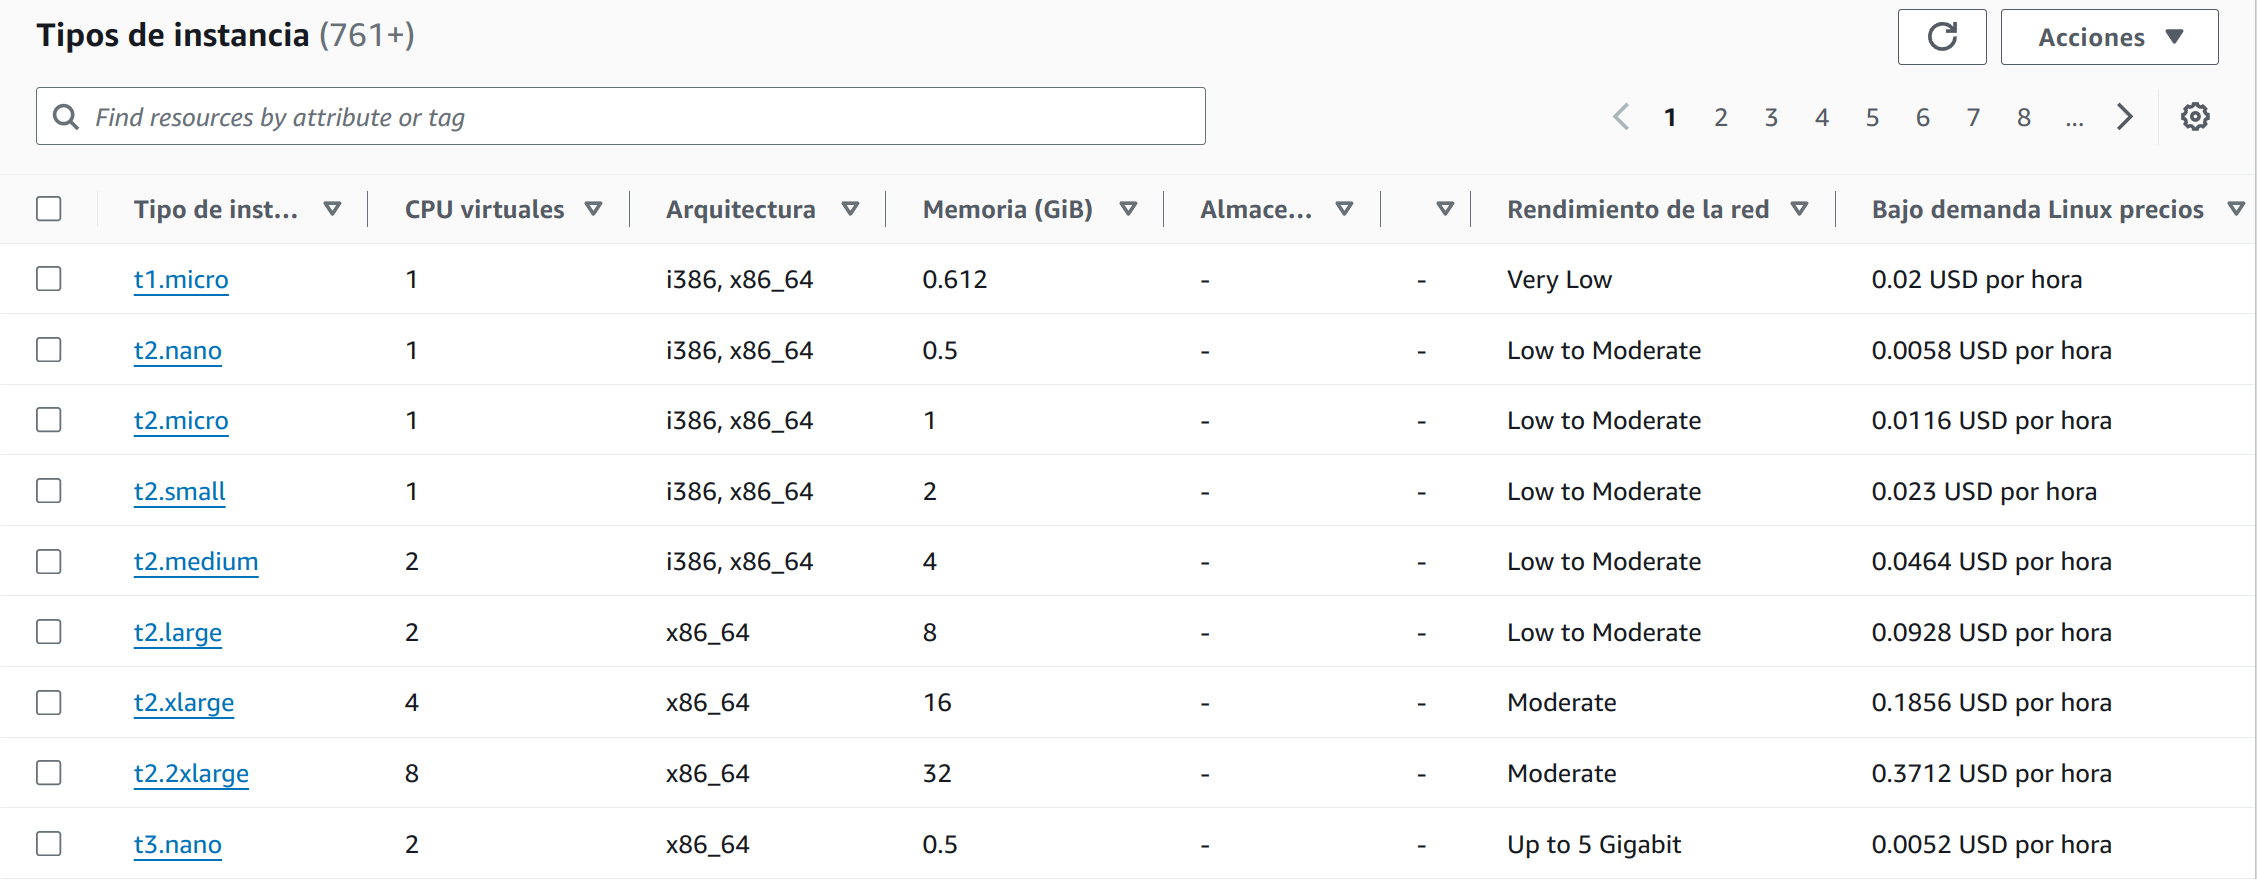
\includegraphics[frame,width=0.8\linewidth]{ec2_instance_types.png}
\end{center}

Los valores que podemos identificar a simple vista son:

\begin{itemize}
	\item \textbf{CPU virtuales}: El número de cores virtuales que el procesador virtual tendrá a su disposición. Dependiendo de nuestras necesidades de cómputo y procesamiento, deberemos elegir un número que se adecúe al rendimiento que esperamos. Actualmente podemos elegir tipos de instancias que tengan entre 1 y 448 CPUs.
	
	\item \textbf{Arquitectura}: Es el tipo de arquitectura del procesador con el que se desplegará la máquina virtual. Entre las arquitecturas que podemos elegir están:
	\begin{itemize}
		\item \textbf{i386}: Arquitectura clásica de equipos de 32 bits.
		\item \textbf{x86\_64}: Arquitectura actual para equipos y servidores.
		\item \textbf{x86\_64\_mac}: Arquitectura utilizada por los equipos Mac con procesadores Intel.
		\item \textbf{arm64}: Arquitectura ARM de 64 bits.
		\item \textbf{arm64\_mac}: Arquitectura ARM de los nuevos procesadores M* de Apple.
	\end{itemize}
	
	\item \textbf{Memoria}: Tamaño de la memoria RAM medido en GiB.
	
	\item \textbf{Rendimiento de la red}: Velocidad de la conexión de red que tendrá la instancia.
	
	\item \textbf{Precio de la instancia}: El coste de la instancia cuando está en funcionamiento se mide en doláres americanos (USD) por hora. El precio varía si el sistema operativo que va a correr la instancia es Linux o Windows, y por supuesto del resto de componentes virtuales.
	
\end{itemize}

\warnbox{\textbf{Se puede cambiar el tipo de instancia, pero para ello se debe parar la instancia}. }


\section{Imágenes AMI}

Una imagen AMI (\textit{Amazon Machine Image})es una plantilla que contiene la configuración del software (el sistema operativo, los servicios y aplicaciones) que son necesarias para correr dentro de nuestra instancia. Existen imágenes AMI públicas creadas por proveedores de software verificados entre las que podremos elegir. 

Hay un catálogo de AMI entre las que podemos elegir:

\begin{itemize}
	\item \textbf{Quickstart AMIs}: Imágenes que normalmente suelen ser el sistema operativo con el mínimo software necesario para hacerlo funcionar. Para correr el resto de servicios, necesitaremos instalar lo que necesitemos.
	
	\item \textbf{Mis AMI}: Podemos crear nuestras propias imágenes para poder reusarlas cuando queramos.
	
	\item \textbf{AMI de AWS Marketplace}: Son imágenes creadas por empresas que pueden contener servicios de alto rendimiento, y \textbf{que en muchos casos pueden ser de pago (por licencia o uso)}.
	
	\item \textbf{AMI de la comunidad}: Imágenes que pueden ser creadas por proveedores oficiales o por comunidades que crean imágenes con software específico.
\end{itemize}

\begin{center}
	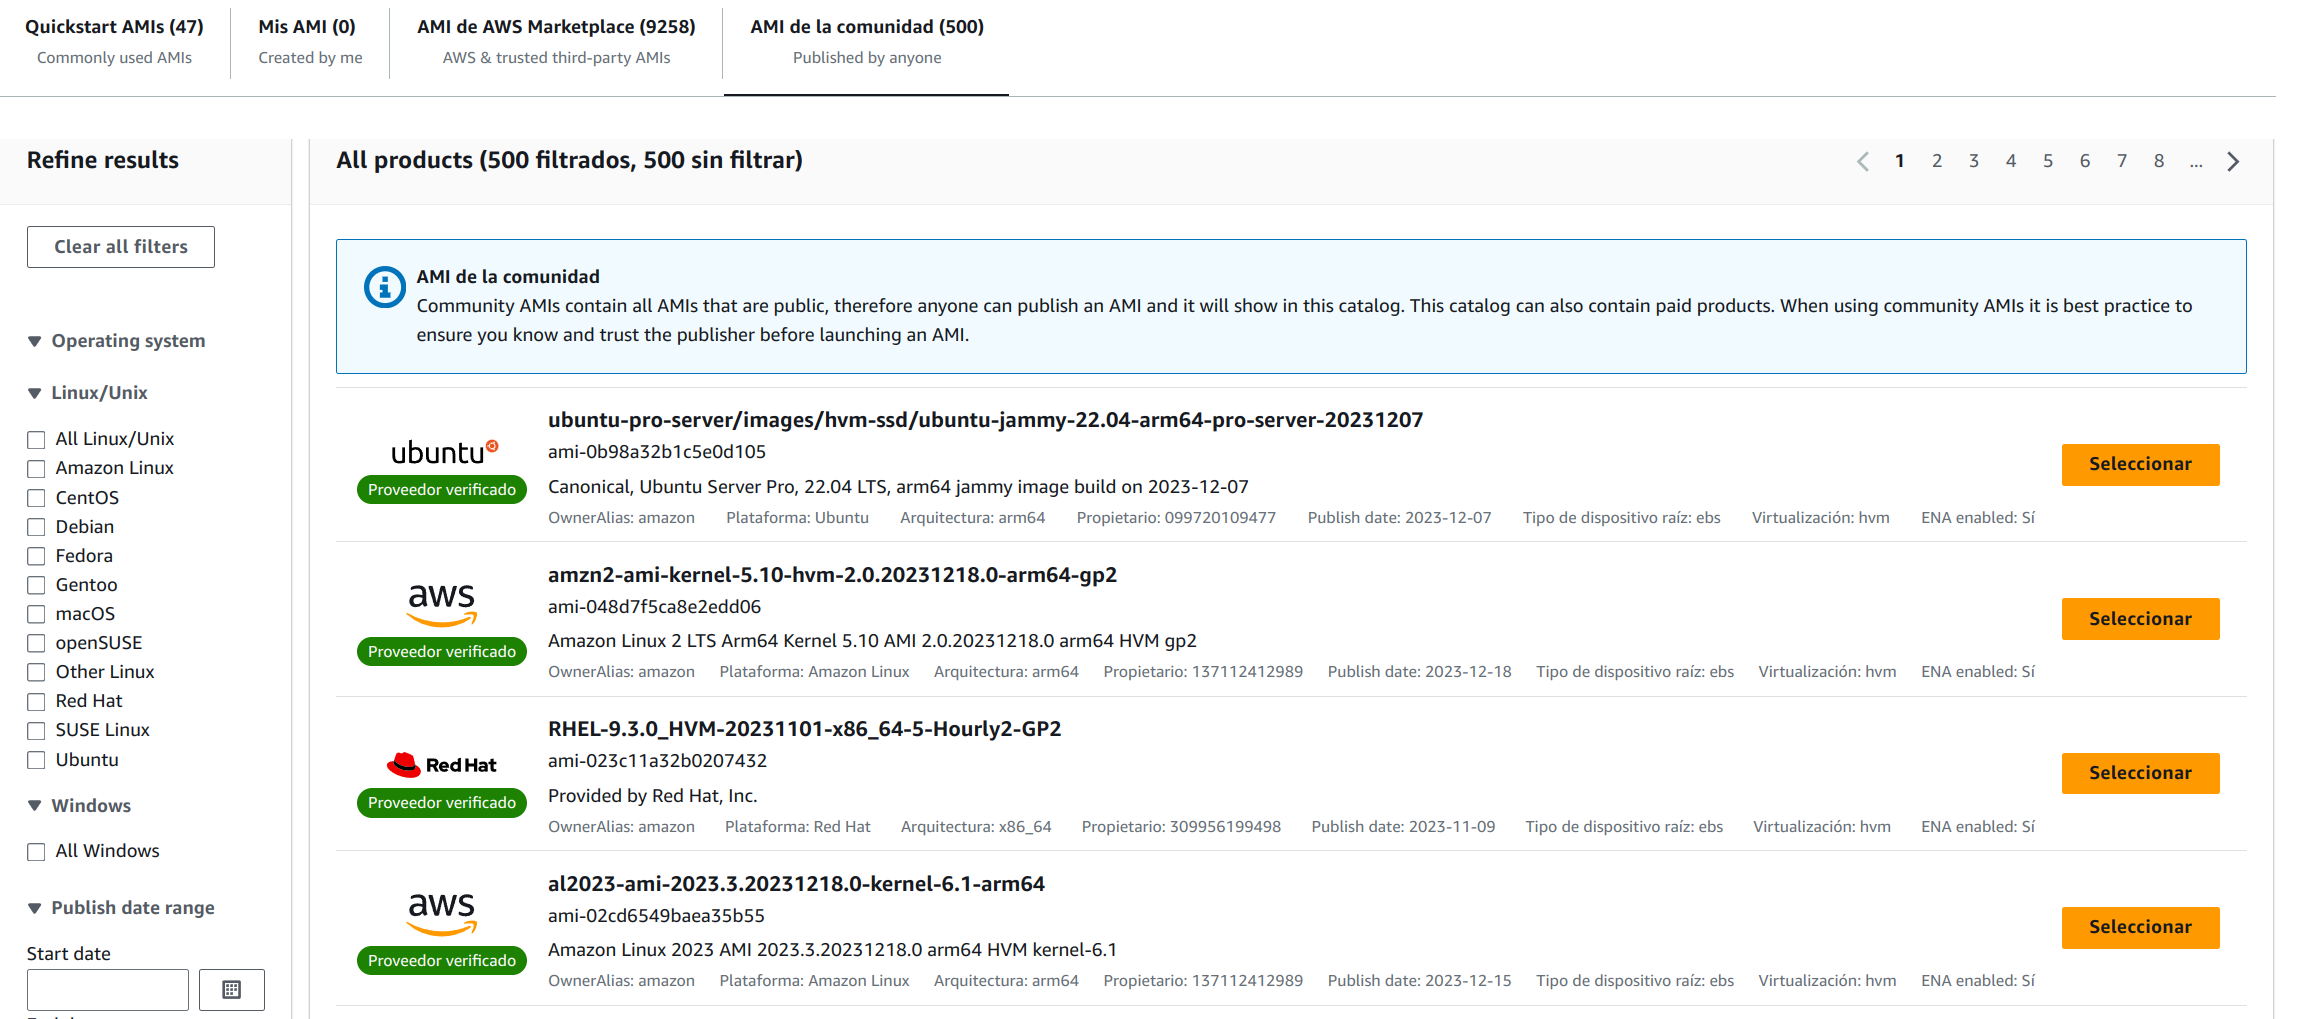
\includegraphics[frame,width=0.9\linewidth]{ec2_ami_catalogue.png}
\end{center}




\infobox{\textbf{Podemos crear nuestras propias imágenes para poder reusarlas cuando queramos.}}

Para empezar, podemos crear nuestra instancia con una imagen AMI de un proveedor oficial, para posteriormente utilizarla como base para crear una AMI propia.


\section{Crear una instancia}

A continuación se va a explicar cómo crear una instancia de tipo Linux teniendo en cuenta todas las posibles opciones que podemos elegir. Para crearla haremos click en 
\includegraphics[height=0.8\baselineskip]{ec2_instance_create.png} y seguiremos las indicaciones para adecuarla a nuestras necesidades.


\chapter{Acceder a una instancia}


\chapter{Security Groups}




